\documentclass[10pt,a4paper]{article}
\usepackage[utf8]{inputenc}
\usepackage[portuguese]{babel}
\usepackage[margin=2cm]{geometry}
\usepackage{multicol}
\usepackage{enumitem}
\usepackage{xcolor}
\usepackage{listings}
\usepackage[box]{automultiplechoice}

% Configuração básica para exibição de códigos
\lstset{
  basicstyle=\small\ttfamily,
  breaklines=true
}

\begin{document}

{
\def\AMCbeginQuestion#1#2{\par\noindent{\bf (POSCOMP 2004 - Questão 02)}}
\begin{question}{} Seja $V$ um espaço vetorial real com produto interno. Para $x$ e $y$ vetores quaisquer de $V$, a igualdade $\|x+y\|=\|x\|+\|y\|$ é verdadeira se, e somente se,
\begin{choices}
\correctchoice{$x=0$, ou $y=0$, ou ($x\neq 0$ e $y=\lambda x$) onde $\lambda$ é um número real não-negativo.}
\wrongchoice{$x\neq 0$ e $y=\lambda x$ para todo número real $\lambda$.}
\wrongchoice{$x=0$, ou $y=0$.}
\wrongchoice{$x=0$, ou $y=0$, ou ($x\neq 0$ e $x,y$ são linearmente dependentes).}
\wrongchoice{$x=0$, ou $y=0$, ou ($x\neq 0$ e $x,y$ são linearmente independentes).}
\end{choices}
\end{question}
}
%
{
\def\AMCbeginQuestion#1#2{\par\noindent{\bf (POSCOMP 2004 - Questão 03)}}
\begin{question}{} Sobre a transformação linear $T:\mathrm{R}^{2}\to\mathrm{R}^{2}$ definida pela matriz $\left[\begin{array}{rr}1&0\\-1&0\end{array}\right]$ podemos dizer que
\begin{choices}
\correctchoice{a imagem é a reta $y=-x$ e o núcleo é a reta $x=0$}
\wrongchoice{a imagem é a reta $y=x$ e o núcleo é $\{(0,0)\}$}
\wrongchoice{a imagem é a reta $x=0$ e o núcleo é a reta $y=-x$}
\wrongchoice{a imagem é a reta $y=x$ e o núcleo é o $\mathrm{R}^{2}$}
\wrongchoice{a imagem é o $\mathrm{R}^{2}$ e o núcleo é a reta $y=x$}
\end{choices}
\end{question}
}
%
{
\def\AMCbeginQuestion#1#2{\par\noindent{\bf (POSCOMP 2004 - Questão 04)}}
\begin{question}{} A transformação $T(x,y)=\frac{1}{5}(-4x+3y,3x+4y)$ do plano no plano é
\begin{choices}
\correctchoice{uma reflexão através da reta $y=3x$}
\wrongchoice{uma expansão uniforme}
\wrongchoice{uma contração uniforme}
\wrongchoice{uma translação}
\wrongchoice{um cisalhamento horizontal}
\end{choices}
\end{question}
}
%
{
\def\AMCbeginQuestion#1#2{\par\noindent{\bf (POSCOMP 2004 - Questão 05)}}
\begin{question}{} No $\mathrm{R}^{3}$ com o produto escalar usual, tome $v=(1,-1,0)$ e o subespaço $S$ gerado por $\{(1,2,1),(-1,1,-1)\}$. O vetor de $S$ mais próximo de $v$ é
\begin{choices}
\correctchoice{$(1/2,-1,1/2)$}
\wrongchoice{$(1,-1,1)$}
\wrongchoice{$(2/3,-1,1/3)$}
\wrongchoice{$(1/100,-1,1/100)$}
\wrongchoice{$(2,-1,2)$}
\end{choices}
\end{question}
}
%
{
\def\AMCbeginQuestion#1#2{\par\noindent{\bf (POSCOMP 2004 - Questão 07)}}
\begin{question}{} Se $A$ é uma matriz $n\times n$ de entradas reais, cujas linhas são linearmente independentes, então não se pode afirmar que:
\begin{choices}
\correctchoice{$\det(A)=1$.}
\wrongchoice{$A$ é inversível.}
\wrongchoice{$A\cdot X=B$ tem solução única $X$ para todo $B\in\mathrm{R}^{n}$.}
\wrongchoice{As colunas de $A$ são linearmente independentes.}
\wrongchoice{O posto de $A$ é $n$.}
\end{choices}
\end{question}
}
%
{
\def\AMCbeginQuestion#1#2{\par\noindent{\bf (POSCOMP 2004 - Questão 18)}}
\begin{question}{} O valor do parâmetro $m$, para que o sistema
\[
\begin{array}{rcl}
x+y+(1-m)z&=&0\\
x+(m-1)y-z&=&0\\
x+my+z&=&0
\end{array}
\]
admita soluções distintas de $(0,0,0)$ é:
\begin{choices}
\correctchoice{$-2$}
\wrongchoice{$-1$}
\wrongchoice{$1$}
\wrongchoice{$2$}
\wrongchoice{$3$}
\end{choices}
\end{question}
}
%
{
\def\AMCbeginQuestion#1#2{\par\noindent{\bf (POSCOMP 2005 - Questão 03)}}
\begin{question}{} Considere a matriz abaixo:
\[
A=\left(\begin{array}{rrrrr}
1&3&1&1&5\\
-2&-6&0&4&-2\\
1&3&2&3&9
\end{array}\right)
\]
O posto de $A$, as dimensões dos dois subespaços: imagem de $A$ e núcleo de $A$, e uma base para a imagem de $A$ são, respectivamente:
\begin{choices}
\correctchoice{$3, 3, 2, \{(1,-2,1),(1,0,2),(1,4,3)\}$}
\wrongchoice{$3, 3, 2, \{(1,-2,1),(1,0,2),(5,-2,9)\}$}
\wrongchoice{$3, 2, 3, \{(1,-2,1),(1,0,2)\}$}
\wrongchoice{$2, 3, 2, \{(1,-2,1),(1,0,2),(5,-2,9)\}$}
\wrongchoice{$2, 3, 2, \{(1,-2,1),(1,0,2)\}$}
\end{choices}
\end{question}
}
%
{
\def\AMCbeginQuestion#1#2{\par\noindent{\bf (POSCOMP 2005 - Questão 04)}}
\begin{question}{} Dada a matriz de transformação linear
\[
A=\left(\begin{array}{rrr}
1&3&2\\
2&1&1\\
3&2&3
\end{array}\right)
\]
pode-se afirmar que:
\begin{choices}
\correctchoice{o vetor $(0,1,0)$ é mapeado para $(3,1,2)$.}
\wrongchoice{o vetor $(1,0,0)$ é mapeado para $(1,3,2)$.}
\wrongchoice{o vetor $(1,0,1)$ é mapeado para $(3,0,2)$.}
\wrongchoice{o vetor $(0,0,1)$ é mapeado para $(3,2,3)$.}
\wrongchoice{o vetor $(1,1,0)$ é mapeado para $(3,2,3)$.}
\end{choices}
\end{question}
}
%
{
\def\AMCbeginQuestion#1#2{\par\noindent{\bf (POSCOMP 2005 - Questão 11)}}
\begin{question}{} Denote por $\langle x,y\rangle$ o produto escalar dos vetores $x=(x_1,x_2,x_3)$ e $y=(y_1,y_2,y_3)$ em $\mathrm{R}^{3}$. O lugar geométrico dado por $\langle x,\mathbf{1}\rangle=r$, onde $\mathbf{1}=(1,1,1)$ e $r\in\mathrm{R}$ é
\begin{choices}
\correctchoice{um plano com vetor normal $\mathbf{1}$}
\wrongchoice{a circunferência de raio $r$ e centro $\mathbf{1}$}
\wrongchoice{um parabolóide com foco em $\mathbf{1}$}
\wrongchoice{um cilindro de raio $r$ e altura $\mathbf{1}$}
\wrongchoice{um hiperbolóide}
\end{choices}
\end{question}
}
%
{
\def\AMCbeginQuestion#1#2{\par\noindent{\bf (POSCOMP 2006 - Questão 13)}}
\begin{question}{} Dados dois vetores no espaço euclidiano $\mathrm{R}^{4}$, $u=(1,3,-2,7)$ e $v=(0,7,2,2)$, pode-se afirmar que:
\begin{choices}
\correctchoice{o quadrado da norma de $v$ é igual a 57}
\wrongchoice{o quadrado da norma de $u$ é igual a 58}
\wrongchoice{o quadrado da distância entre $u$ e $v$ é dado por 63}
\wrongchoice{os vetores $u$ e $v$ são ortogonais}
\wrongchoice{nenhuma das anteriores}
\end{choices}
\end{question}
}
%
{
\def\AMCbeginQuestion#1#2{\par\noindent{\bf (POSCOMP 2006 - Questão 14)}}
\begin{question}{} Uma condição necessária e suficiente para que o sistema $Ax=b$ tenha solução única é:
\begin{choices}
\correctchoice{As colunas de $A$ são vetores linearmente independentes que geram um subespaço contendo $b$.}
\wrongchoice{$Ax=0$ tem solução única.}
\wrongchoice{As linhas de $A$ são vetores linearmente independentes.}
\wrongchoice{A matriz $A$ é quadrada e não-singular.}
\wrongchoice{O posto de $A$ é igual a seu número de linhas.}
\end{choices}
\end{question}
}
%
{
\def\AMCbeginQuestion#1#2{\par\noindent{\bf (POSCOMP 2006 - Questão 15)}}
\begin{question}{} Não é correto afirmar que:
\begin{choices}
\wrongchoice{Se as colunas de uma matriz são vetores dois a dois ortogonais, então sua inversa é sua transposta.}
\wrongchoice{Se a inversa de uma matriz é ela própria, então toda potência dessa matriz é ela própria ou a identidade.}
\wrongchoice{Se uma matriz singular é o produto de duas outras matrizes quadradas, então uma destas também é singular.}
\correctchoice{Se três matrizes quadradas $A$, $B$ e $C$ satisfazem $A(B-C)=0$, então $A=0$ ou $B=C$.}
\wrongchoice{Se $A$ e $B$ são matrizes triangulares inferiores então $AB$ também é triangular inferior.}
\end{choices}
\end{question}
}
%
{
\def\AMCbeginQuestion#1#2{\par\noindent{\bf (POSCOMP 2007 - Questão 03)}}
\begin{question}{} Com respeito a uma matriz quadrada $A$ de ordem $n$, com entradas reais, as assertivas abaixo são equivalentes a dizer que $A$ tem inversa, EXCETO
\begin{choices}
\correctchoice{dois-a-dois os vetores-coluna de $A$ não podem ser colineares.}
\wrongchoice{as linhas de $A$ são vetores linearmente independentes.}
\wrongchoice{o sistema $Ax=0$ tem solução única.}
\wrongchoice{o determinante da transposta de $A$ é diferente de zero.}
\wrongchoice{o sistema $Ax=b$ tem solução única para qualquer vetor $n$-dimensional $b$.}
\end{choices}
\end{question}
}
%
{
\def\AMCbeginQuestion#1#2{\par\noindent{\bf (POSCOMP 2007 - Questão 04)}}
\begin{question}{} É CORRETO afirmar
\begin{choices}
\correctchoice{que, se $u$ e $v$ são vetores não-nulos de $\mathrm{R}^{n}$, então $u$ é autovetor da matriz $uv^{T}$.}
\wrongchoice{que os autovalores de uma matriz não-singular são positivos.}
\wrongchoice{que, para uma matriz $A$, $\lambda$ é autovalor de $A$ se, e somente se, $\lambda^{2}$ é um autovalor de $A^{2}$.}
\wrongchoice{que, se uma matriz é igual a sua inversa, então seus autovalores são iguais a 1.}
\wrongchoice{que, se uma matriz quadrada tem entradas reais, então seus autovalores são números reais.}
\end{choices}
\end{question}
}
%
{
\def\AMCbeginQuestion#1#2{\par\noindent{\bf (POSCOMP 2007 - Questão 05)}}
\begin{question}{} Dados dois vetores $\vec{u}$ e $\vec{v}\in\mathrm{R}^{2}$, o vetor $\vec{u}$ tem origem em $(-1,4)$ e extremidade em $(3,5)$ e o vetor $\vec{v}$ é igual a $(-10,7)$. Considere $\vec{w}$ o vetor em $\mathrm{R}^{2}$ que apresenta comprimento igual a 5 e é perpendicular à soma dos vetores $\vec{u}$ e $\vec{v}$. Nesse caso, o vetor $\vec{w}$ pode ser expresso por
\begin{choices}
\correctchoice{$(-3,-4)$}
\wrongchoice{$(3,4)$}
\wrongchoice{$(3,-4)$}
\wrongchoice{$(-4,3)$}
\wrongchoice{$(4,3)$}
\end{choices}
\end{question}
}
%
{
\def\AMCbeginQuestion#1#2{\par\noindent{\bf (POSCOMP 2009 - Questão 01)}}
\begin{question}{} Seja $F$ uma transformação linear de $\mathrm{R}^{2}$ em $\mathrm{R}^{2}$ que transforma o vetor genérico $(x,y)^{T}$ em $(y,x)^{T}$. Seja $A$ a matriz associada a $F$ e seja $B$ a matriz associada a $F^{-1}$, a transformação inversa de $F$.

Considere as seguintes afirmativas:
\begin{enumerate}
\item[I.] $B=\left[\begin{array}{rr}0&1\\1&0\end{array}\right]$
\item[II.] $A=-B$
\item[III.] A transformação linear $G$ que transforma o vetor genérico $(x,y)^{T}$ em $(0,y)^{T}$ não possui transformação inversa.
\end{enumerate}
Assinale a alternativa CORRETA:
\begin{choices}
\correctchoice{Apenas a afirmativa II é FALSA.}
\wrongchoice{Apenas a afirmativa I é CORRETA.}
\wrongchoice{Apenas a afirmativa III é CORRETA.}
\wrongchoice{Todas as afirmativas são corretas.}
\wrongchoice{Todas as afirmativas são falsas.}
\end{choices}
\end{question}
}
%
{
\def\AMCbeginQuestion#1#2{\par\noindent{\bf (POSCOMP 2009 - Questão 02)}}
\begin{question}{} Dadas as matrizes $A=\left[\begin{array}{rr}1&2\\3&4\end{array}\right]$, $B=\left[\begin{array}{rr}5&6\\7&8\end{array}\right]$ e $C=\left[\begin{array}{rr}1&3\\5&2\end{array}\right]$, o resultado de $A\times B+C^{T}$ é:
\begin{choices}
\correctchoice{$\left[\begin{array}{rr}20&27\\46&52\end{array}\right]$}
\wrongchoice{$\left[\begin{array}{rr}20&25\\48&52\end{array}\right]$}
\wrongchoice{$\left[\begin{array}{rr}19&22\\43&50\end{array}\right]$}
\wrongchoice{$\left[\begin{array}{rr}24&39\\34&48\end{array}\right]$}
\wrongchoice{Nenhuma das respostas anteriores.}
\end{choices}
\end{question}
}
%
{
\def\AMCbeginQuestion#1#2{\par\noindent{\bf (POSCOMP 2010 - Questão 01)}}
\begin{question}{} Considere a matriz
\[
A=\left[\begin{array}{rrr}4&-3&1\\2&-1&1\\0&0&2\end{array}\right]
\]
Os autovalores da matriz $A$ são:
\begin{choices}
\correctchoice{$1, 2, 2$}
\wrongchoice{$0, 1, 4$}
\wrongchoice{$0, 2, 3$}
\wrongchoice{$1, 1, 3$}
\wrongchoice{$2, 3, -1$}
\end{choices}
\end{question}
}
%
{
\def\AMCbeginQuestion#1#2{\par\noindent{\bf (POSCOMP 2010 - Questão 03)}}
\begin{question}{} Seja
\[
A=\left[\begin{array}{rrr}1&-1&1\\2&-2&1\\2&-2&1\end{array}\right].
\]
Então $A^{7}$ vale:
\begin{choices}
\correctchoice{$\left[\begin{array}{rrr}1&-1&1\\2&-2&1\\2&-2&1\end{array}\right]$}
\wrongchoice{$\left[\begin{array}{rrr}10&-1&2\\2&-2&3\\2&-2&5\end{array}\right]$}
\wrongchoice{$\left[\begin{array}{rrr}1&-1&1\\27&-27&1\\27&-27&1\end{array}\right]$}
\wrongchoice{$\left[\begin{array}{rrr}1&-1&1\\16&-21&1\\34&-64&1\end{array}\right]$}
\wrongchoice{$\left[\begin{array}{rrr}-1&1&-1\\-2&2&-1\\-2&2&-1\end{array}\right]$}
\end{choices}
\end{question}
}
%
{
\def\AMCbeginQuestion#1#2{\par\noindent{\bf (POSCOMP 2010 - Questão 05)}}
\begin{question}{} Considere os conjuntos de polinômios $A=\{1,x,3x^{2}-1,5x^{3}-3\}$ e $B=\{1,x,x^{2},x^{3}\}$ e o produto interno $\langle p,q\rangle=\int_{-1}^{1}p(x)q(x)\,dx$.
Com base no enunciado, considere as afirmativas a seguir.
\begin{enumerate}
\item[I.] $A$ é um conjunto linearmente independente.
\item[II.] $B$ é um conjunto linearmente independente.
\item[III.] $A$ é a base ortogonal do conjunto de polinômios de grau até 3.
\item[IV.] $B$ é a base ortogonal do conjunto de polinômios de grau até 3.
\end{enumerate}
Assinale a alternativa correta.
\begin{choices}
\correctchoice{Somente as afirmativas I e II são corretas.}
\wrongchoice{Somente as afirmativas I e IV são corretas.}
\wrongchoice{Somente as afirmativas III e IV são corretas.}
\wrongchoice{Somente as afirmativas I, II e III são corretas.}
\wrongchoice{Somente as afirmativas II, III e IV são corretas.}
\end{choices}
\end{question}
}
%
{
\def\AMCbeginQuestion#1#2{\par\noindent{\bf (POSCOMP 2011 - Questão 01)}}
\begin{question}{} Considere a matriz a seguir.
\[
A=\left[\begin{array}{rrr}2&4&2\\1&5&2\\4&-1&9\end{array}\right]
\]
No método da eliminação de Gauss, foram efetuados os seguintes passos para se obter uma matriz na forma degrau:
\begin{enumerate}
\item[I.] Subtraiu-se a metade da primeira linha da segunda.
\item[II.] Subtraiu-se o dobro da primeira linha da terceira.
\item[III.] Adicionou-se o triplo da segunda linha à terceira.
\end{enumerate}
Em termos matriciais, o processo descrito corresponde a:
\begin{choices}
\correctchoice{Multiplicar $A$, à esquerda, por $\left[\begin{array}{rrr}1&0&0\\-1/2&1&0\\-7/2&3&1\end{array}\right]$}
\wrongchoice{Adicionar à $A$ a matriz $\left[\begin{array}{rrr}0&0&0\\-1&-2&0\\-4&1&1\end{array}\right]$}
\wrongchoice{Multiplicar $A$, à esquerda, por $\left[\begin{array}{rrr}0&0&0\\2&0&0\\1/2&-1/3&0\end{array}\right]$}
\wrongchoice{Multiplicar $A$, à direita, por $\left[\begin{array}{rrr}1&-1/2&-2\\0&1&-3\\0&0&1\end{array}\right]$}
\wrongchoice{Subtrair de $A$ a matriz $\left[\begin{array}{rrr}2&4&2\\0&5&2\\0&0&9\end{array}\right]$}
\end{choices}
\end{question}
}
%
{
\def\AMCbeginQuestion#1#2{\par\noindent{\bf (POSCOMP 2011 - Questão 03)}}
\begin{question}{} Suponha que, em vez de usar a base padrão $\{e_1,e_2\}$ para $\mathrm{R}^{2}$, onde $e_1=[1,0]^{T}$ e $e_2=[0,1]^{T}$, deseja-se utilizar a base $\{u_1,u_2\}$, com $u_1=[3,2]^{T}$ e $u_2=[1,1]^{T}$. As coordenadas do vetor $x=[7,4]^{T}$ em relação a $u_1$ e $u_2$ são:
\begin{choices}
\correctchoice{$[3,-2]^{T}$}
\wrongchoice{$[0,1]^{T}$}
\wrongchoice{$[1,-2]^{T}$}
\wrongchoice{$[4,3]^{T}$}
\wrongchoice{$[15,18]^{T}$}
\end{choices}
\end{question}
}
%
{
\def\AMCbeginQuestion#1#2{\par\noindent{\bf (POSCOMP 2011 - Questão 06)}}
\begin{question}{} O problema de determinar um vetor normal a um triângulo ou polígono é muito comum em computação gráfica. Dado o triângulo formado pelos pontos $A(1,2,3)$, $B(3,2,1)$ e $C(1,1,1)$, um vetor normal, $n$, a esse triângulo é dado por:
\begin{choices}
\correctchoice{$n=[-2,4,-2]^{T}$}
\wrongchoice{$n=[0,0,4]^{T}$}
\wrongchoice{$n=[2,-1,-4]^{T}$}
\wrongchoice{$n=[3,4,5]^{T}$}
\wrongchoice{$n=[5,5,5]^{T}$}
\end{choices}
\end{question}
}
%
{
\def\AMCbeginQuestion#1#2{\par\noindent{\bf (POSCOMP 2012 - Questão 01)}}
\begin{question}{} Com base no sistema de equações de variáveis $x$, $y$ e $z$ dado por
\[
\begin{array}{rcl}
xy-2\sqrt{y}+3yz&=&8\\
2xy-3\sqrt{y}+2yz&=&7\\
-xy+\sqrt{y}+2yz&=&4
\end{array}
\]
considere as afirmativas a seguir.
\begin{enumerate}
\item[I.] O sistema é possível e determinado.
\item[II.] O posto da matriz ampliada do sistema é 2.
\item[III.] Na matriz transposta dos coeficientes associada ao sistema $a_{12}=-3$.
\item[IV.] A matriz dos coeficientes associada ao sistema é inversível.
\end{enumerate}
Assinale a alternativa correta.
\begin{choices}
\correctchoice{Somente as afirmativas I e IV são corretas.}
\wrongchoice{Somente as afirmativas I e II são corretas.}
\wrongchoice{Somente as afirmativas III e IV são corretas.}
\wrongchoice{Somente as afirmativas I, II e III são corretas.}
\wrongchoice{Somente as afirmativas II, III e IV são corretas.}
\end{choices}
\end{question}
}
%
{
\def\AMCbeginQuestion#1#2{\par\noindent{\bf (POSCOMP 2012 - Questão 02)}}
\begin{question}{} Seja o espaço vetorial $V=\mathrm{R}^{2}$. Com relação a esse espaço, assinale a alternativa correta.
\begin{choices}
\correctchoice{$V$ é soma direta de $S_1=\{(x,y)\in\mathrm{R}^{2}\mid(x,y)=(x,0)\}$ e $S_2=\{(x,y)\in\mathrm{R}^{2}\mid(x,y)=(0,y)\}$, ou seja, $V=S_1\oplus S_2$.}
\wrongchoice{$S=\{(x,y)\in\mathrm{R}^{2}\mid y=2x-1\}$ é um subespaço vetorial de $V$.}
\wrongchoice{O conjunto $\{(1,2),(2,4)\}$ é base de $V$.}
\wrongchoice{Existem vetores $u,v$ em $V$ tais que $u+v\neq v+u$.}
\wrongchoice{Se $S_1$ e $S_2$ são dois subespaços quaisquer de $V$, então vale a relação: $(\mbox{dimensão de }S_1+\mbox{dimensão de }S_2-\mbox{dimensão de }S_1\cap S_2)>2$.}
\end{choices}
\end{question}
}
%
{
\def\AMCbeginQuestion#1#2{\par\noindent{\bf (POSCOMP 2012 - Questão 05)}}
\begin{question}{} Uma rotação que gira cada vetor em $\mathrm{R}^{2}$ por um ângulo fixado, no sentido anti-horário, é uma transformação linear, conforme ilustra a figura a seguir.
\begin{center}
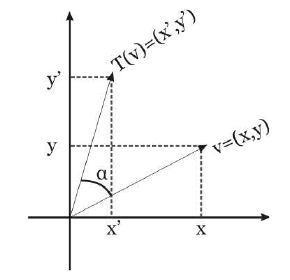
\includegraphics[width=0.27\textwidth]{poscomp_2012_q05_figura.png}
\end{center}
Seja $T:\mathrm{R}^{2}\to\mathrm{R}^{2}$ uma rotação. Se $T(4,2)=(-2,4)$, assinale a alternativa que apresenta, corretamente, o valor do ângulo $\alpha$.
\begin{choices}
\correctchoice{$\pi/2$}
\wrongchoice{$\pi/6$}
\wrongchoice{$\pi/4$}
\wrongchoice{$\pi/3$}
\wrongchoice{$\pi$}
\end{choices}
\end{question}
}
%
{
\def\AMCbeginQuestion#1#2{\par\noindent{\bf (POSCOMP 2012 - Questão 08)}}
\begin{question}{} Considere $u$ e $v$ dois vetores em $\mathrm{R}^{2}$. Com relação a esses vetores, assinale a alternativa correta.
\begin{choices}
\correctchoice{Os vetores $u$ e $v$ são perpendiculares se, e somente se, seu produto escalar $u\cdot v=0$.}
\wrongchoice{O vetor $ku$, com $k\in\mathrm{R}$, é um vetor que tem o mesmo sentido do vetor $u$.}
\wrongchoice{Se $u=(2,3)$ e $v=(1,5)$ então o produto escalar $u\cdot v=15$.}
\wrongchoice{Se $u=(x_1,y_1)$ e $v=(x_2,y_2)$ então $|u+v|<|u|$.}
\wrongchoice{Se $u=(-2,-2)$ e $v=(0,-2)$ então o ângulo entre $u$ e $v$ é $\pi/6$.}
\end{choices}
\end{question}
}
%
{
\def\AMCbeginQuestion#1#2{\par\noindent{\bf (POSCOMP 2013 - Questão 02)}}
\begin{question}{} Com relação à matriz $A=\left[\begin{array}{rrr}2&1&0\\1&0&2\\0&2&1\end{array}\right]$, considere as afirmativas a seguir.
\begin{enumerate}
\item[I.] Um autovetor associado à $A$ é $v=(x,2x,-x)$, com $x\neq0$.
\item[II.] Os autovalores de $A$ são 1, $-3$ e $-1$.
\item[III.] A matriz inversa de $A$ é $\left[\begin{array}{rrr}4/9&1/9&-2/9\\1/9&-2/9&4/9\\-2/9&4/9&1/9\end{array}\right]$.
\item[IV.] Os polinômios característico e minimal associados à $A$ são iguais.
\end{enumerate}
Assinale a alternativa correta.
\begin{choices}
\correctchoice{Somente as afirmativas III e IV são corretas.}
\wrongchoice{Somente as afirmativas I e II são corretas.}
\wrongchoice{Somente as afirmativas I e IV são corretas.}
\wrongchoice{Somente as afirmativas I, II e III são corretas.}
\wrongchoice{Somente as afirmativas II, III e IV são corretas.}
\end{choices}
\end{question}
}
%
{
\def\AMCbeginQuestion#1#2{\par\noindent{\bf (POSCOMP 2013 - Questão 03)}}
\begin{question}{} Considere o sistema linear a seguir.
\[
\begin{array}{rcl}3x+y+z&=&2\\5x+3y+2z&=&5\\7x+7y+8z&=&15\end{array}
\]
A solução desse sistema é interpretada, geometricamente, por
\begin{choices}
\correctchoice{três planos distintos cruzando-se em um único ponto.}
\wrongchoice{dois planos paralelos e um plano cruzando-os.}
\wrongchoice{três planos paralelos coincidentes.}
\wrongchoice{três planos paralelos, sendo dois coincidentes e um concorrente.}
\wrongchoice{três planos distintos cruzando-se em uma única reta.}
\end{choices}
\end{question}
}
%
{
\def\AMCbeginQuestion#1#2{\par\noindent{\bf (POSCOMP 2013 - Questão 05)}}
\begin{question}{} Considerando a transformação linear do plano $T(x,y)=(15x+y,34x+27y)$, assinale a alternativa correta.
\begin{choices}
\correctchoice{$T$ é inversível.}
\wrongchoice{A dimensão do núcleo de $T$ é igual a 1.}
\wrongchoice{Existem $(a,b)$ e $(c,d)$ distintos tais que $T(a,b)=T(c,d)$.}
\wrongchoice{Imagem de $T$ é diferente de $\mathrm{R}^{2}$.}
\wrongchoice{O núcleo de $T$ é diferente de 0.}
\end{choices}
\end{question}
}
%
{
\def\AMCbeginQuestion#1#2{\par\noindent{\bf (POSCOMP 2013 - Questão 06)}}
\begin{question}{} Com relação ao produto vetorial no espaço $\mathrm{R}^{3}$, assinale a alternativa correta.
\begin{choices}
\correctchoice{Vale a propriedade distributiva em relação à adição de vetores.}
\wrongchoice{Vale a lei do cancelamento para produtos vetoriais.}
\wrongchoice{Vale a propriedade associativa.}
\wrongchoice{Vale a propriedade comutativa.}
\wrongchoice{Se o produto vetorial entre dois vetores é nulo, então esses vetores são nulos.}
\end{choices}
\end{question}
}
%
{
\def\AMCbeginQuestion#1#2{\par\noindent{\bf (POSCOMP 2013 - Questão 08)}}
\begin{question}{} Com relação ao conjunto $B=\{(1,2),(3,4)\}$ do plano cartesiano e ao produto interno usual do plano, considere as afirmativas a seguir.
\begin{enumerate}
\item[I.] $B$ é uma base do plano cartesiano.
\item[II.] Bases têm apenas coordenadas 0 ou 1.
\item[III.] $B$ é uma base ortogonal do plano.
\item[IV.] Uma base ortonormal a $B$ é $\left\{\left(\frac{1}{\sqrt5},\frac{2}{\sqrt5}\right),\left(\frac{2}{\sqrt5},-\frac{1}{\sqrt5}\right)\right\}$.
\end{enumerate}
Assinale a alternativa correta.
\begin{choices}
\correctchoice{Somente as afirmativas I e IV são corretas.}
\wrongchoice{Somente as afirmativas I e II são corretas.}
\wrongchoice{Somente as afirmativas III e IV são corretas.}
\wrongchoice{Somente as afirmativas I, II e III são corretas.}
\wrongchoice{Somente as afirmativas II, III e IV são corretas.}
\end{choices}
\end{question}
}
%
{
\def\AMCbeginQuestion#1#2{\par\noindent{\bf (POSCOMP 2013 - Questão 09)}}
\begin{question}{} Considere a reta $t$ com vetor diretor $\vec t$ e o plano $\alpha$ determinado pelos vetores $\vec a$ e $\vec b$. Supondo que $\vec t$, $\vec a$ e $\vec b$ são vetores linearmente independentes, assinale a alternativa correta.
\begin{choices}
\correctchoice{A reta $t$ e o plano $\alpha$ são transversais.}
\wrongchoice{A reta $t$ e o plano $\alpha$ são paralelos.}
\wrongchoice{A reta $t$ pertence ao plano $\alpha$.}
\wrongchoice{O vetor $\vec t$ é uma combinação linear de $\vec a$ e $\vec b$.}
\wrongchoice{Os vetores $\vec t$ e $-\vec t$ são linearmente independentes.}
\end{choices}
\end{question}
}
%

\end{document}
